\documentclass[a4]{article}

\usepackage[left=3cm,right=3cm,top=2cm,bottom=2cm]{geometry} 

\usepackage[utf8]{inputenc}   % otra alternativa para los caracteres acentuados y la "ñ"
\usepackage[           spanish % para poder usar el español
                      ,es-tabla % para los captions de las tablas
                       ]{babel}   
%\decimalpoint %para usar el punto decimal en vez de coma para los números con decimales

\usepackage[T1]{fontenc}
\usepackage{lmodern}

\usepackage{parskip}
\usepackage{xcolor}

\usepackage{caption}
\usepackage{hyperref}
\usepackage{enumerate} % paquete para poder personalizar fácilmente la apariencia de las listas enumerativas
\usepackage{listings}
\usepackage{xcolor}
\usepackage{amsmath}
\definecolor{codegreen}{rgb}{0,0.6,0}
\definecolor{codegray}{rgb}{0.2,0.2,0.2}
\definecolor{codepurple}{rgb}{0.58,0,0.82}
\definecolor{backcolour}{rgb}{0.95,0.95,0.92}

\lstdefinestyle{mystyle}{
	backgroundcolor=\color{backcolour},   
	commentstyle=\color{codegray},
	keywordstyle=\color{codegreen},
	numberstyle=\tiny\color{blue},
	stringstyle=\color{red},
	basicstyle=\ttfamily\normalsize,
	breakatwhitespace=false,         
	breaklines=true,                 
	captionpos=b,                    
	keepspaces=true,                 
	numbers=left,                    
	numbersep=5pt,                  
	showspaces=false,                
	showstringspaces=false,
	showtabs=false,                  
	tabsize=2
}

\lstset{style=mystyle}
\usepackage{graphicx} % figuras
\usepackage{subfigure} % subfiguras

\usepackage{amsfonts}
\usepackage{amsmath}

\definecolor{gris}{RGB}{220,220,220}
	
\usepackage{float} % para controlar la situación de los entornos flotantes

\restylefloat{figure}
\restylefloat{table} 

\newcommand{\HRule}{\rule{\linewidth}{0.5mm}}

\author{Pilar Navarro Ramírez}
\date{\vspace{-5mm}}

\title{\huge APRENDIZAJE AUTOMÁTICO: Práctica 1 \HRule\vspace{-4mm}}

\begin{document}
\maketitle
\tableofcontents

\newpage

\section{Ejercicio sobre la búsqueda iterativa de óptimos:\\ Gradiente descendente}

\subsection{Ejercicio 1}
\textbf{Implementar el algoritmo de gradiente descendente}

Vamos a usar el algoritmo de gradiente descendente para buscar mínimos de funciones. Este algoritmo es el siguiente:

\begin{lstlisting}[language=Python]
Gradiente Descendente:
	w <-- punto inicial
	for i in range(max_iteraciones):
		w <-- (w - learning_rate*gradiente(w))
	return w
\end{lstlisting}
donde w son las coordenadas que se obtienen en cada iteración del algoritmo

El algoritmo parte de un punto inicial, unas coordenadas. En cada iteración estas se desplazan en la dirección opuesta al gradiente (de la función de estudio) en ese punto y lo hacen una cantidad proporcional al gradiente indicada por el parámetro de learning rate, o tasa de aprendizaje. El algoritmo se repite durante un determinado número de iteraciones, parámetro que establece el programador, y al final devuelve las coordenadas encontradas en la última iteración. 

A lo largo de la práctica implementamos este algoritmo en distintas funciones, a saber:\\ \lstinline{gradient_descent(init,f,grad,error2get,maxIter,lr), gd(init,f,grad,maxIter,lr)} y\\
\lstinline{plot_gd(init,f,grad,maxIter,lr)}.
\subsection{Ejercicio 2}
\textbf{Considerar la función $E(u, v) = (u^3e^{(v-2)} - 2v^2e^{-u} )^2$ . Usar gradiente descendente
para encontrar un mínimo de esta función, comenzando desde el punto $(u, v) = (1, 1)$ y
usando una tasa de aprendizaje de $\eta = 0.1$.}

\subsubsection{Apartado a)}
\textbf{Calcular analíticamente y mostrar la expresión del gradiente de la función $E(u, v)$}

En primer lugar calculamos las derivadas parciales de $E(u, v)$:
 \[
\frac{\partial E}{\partial u}(u,v) =
2(u^3e^{(v-2)} - 2v^2e^{-u})(3u^2e^{(v-2)} + 2v^2e^{-u})
\]

y

\[
\frac{\partial E}{\partial v}(u,v) =
2(u^3e^{(v-2)} - 2v^2e^{-u})(u^3e^{(v-2)} - 4ve^{-u})
\]

En el código las derivadas parciales están definidas por las funciones \lstinline|dEu| (derivada parcial con respecto a la primera variable) y \lstinline|dEv| (derivada parcial con respecto a la segunda variable).

Una vez que tenemos las derivadas parciales, conocemos el gradiente de la función considerada, que es el siguiente:
\begin{align*}
\nabla E(u,v) & = (\frac{\partial E}{\partial u}(u,v),\frac{\partial E}{\partial v}(u,v))=\\
& = (2(u^3e^{(v-2)} - 2v^2e^{-u})(3u^2e^{(v-2)} + 2v^2e^{-u}), 2(u^3e^{(v-2)} - 2v^2e^{-u})(u^3e^{(v-2)} - 4ve^{-u}))
\end{align*}

La función \lstinline|gradE| devuelve el gradiente de $E(u,v)$ en el punto que se pase como parámetro.

\subsubsection{Apartado b)}
\textbf{¿Cuántas iteraciones tarda el algoritmo en obtener por primera vez un valor de E(u, v)
inferior a $10^{-14}$?}

Vamos a aplicar el algoritmo de gradiente descendente, explicado en el ejercicio 1, para minimizar la función  $E(u,v)$, que tiene la siguiente forma:
\begin{figure}[H]
	\centering
	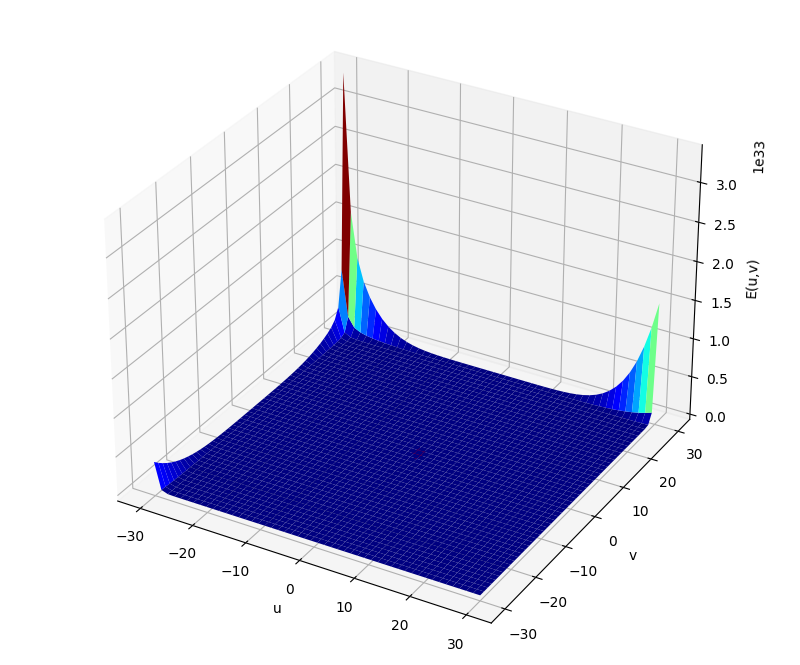
\includegraphics[width=0.8\linewidth]{img/Figure_1}
	\caption{}
	\label{fig:figure1}
\end{figure}


Podemos ver en la figura que esta función sólo tiene un mínimo, luego podemos asegurar que si el algoritmo encuentra un mínimo será el mínimo global. En él la función toma el valor 0, por lo que buscamos un 0 de $E$. Así pues, debemos aplicar el algoritmo hasta encontrar un punto en el que la función sea 0. Pero, como el 0 absoluto no se puede alcanzar (en el ordenador), consideramos un margen de eror de $\varepsilon=10^{-14}$ (\lstinline|error2get|), esto es, iteramos hasta que la función tome un valor menor o igual a $\varepsilon$.

Para ello, partimos del punto $w:=(u,v)=(1,1)$ (\lstinline|init|) y tomamos como tasa de aprendizaje \\ $\eta=0.1$ (\lstinline|lr|). Además, vamos a considerar un máximo número de iteraciones (\lstinline|maxIter|) de 100 (pues no necesitamos más, como vamos a ver a continuación), para tener un criterio de parada en caso de que el algoritmo no encontrase nunca el mínimo. 

Todo este proceso es llevado a cabo por la función \lstinline|gradient_descent(init,f,grad,error2get,maxIter,lr)|.
Tras ejecutarla para \lstinline|f=E| y \lstinline|grad=gradE|, con los valores del resto de parámetros ya indicados, descubrimos que el mínimo \underline{se encuentra en solo 10 iteraciones}. 

\subsubsection{Apartado c)}

\textbf{¿En qué coordenadas $(u,v)$ se alcanzó por primera vez un valor igual o menor a $10^{-14}$
en el apartado anterior?}

En las coordenadas $( 1.1572888496465497 ,  0.9108383657484799 )$ se alcanza por primera vez un valor menor a $10^{-14}$. En concreto, el valor de $E(u,v)$ en este punto es de $3.1139605842768533\cdot10^{-15}$.

\subsection{Ejercicio 3}

\textbf{Considerar ahora la función $f(x,y)=(x+2)^2 +2(y-2)^2 +2\sin(2\pi x)sin(2\pi y)$.}

\subsubsection{Apartado a)}

\textbf{Usar gradiente descendente para minimizar esta función. Usar como punto inicial \\ $(x_0=-1,y_0=1)$, tasa de aprendizaje $\eta = 0.01$ y un máximo de 50 iteraciones.
Generar un gráfico de cómo desciende el valor de la función con las iteraciones. Repetir el experimento pero usando $\eta = 0.1$ comentar las diferencias y su dependencia de $\eta$}

Empezamos viendo la forma de la función considerada $f(x,y)$:
\begin{figure}[H]
	\centering    
	\subfigure[Vista general de la función]{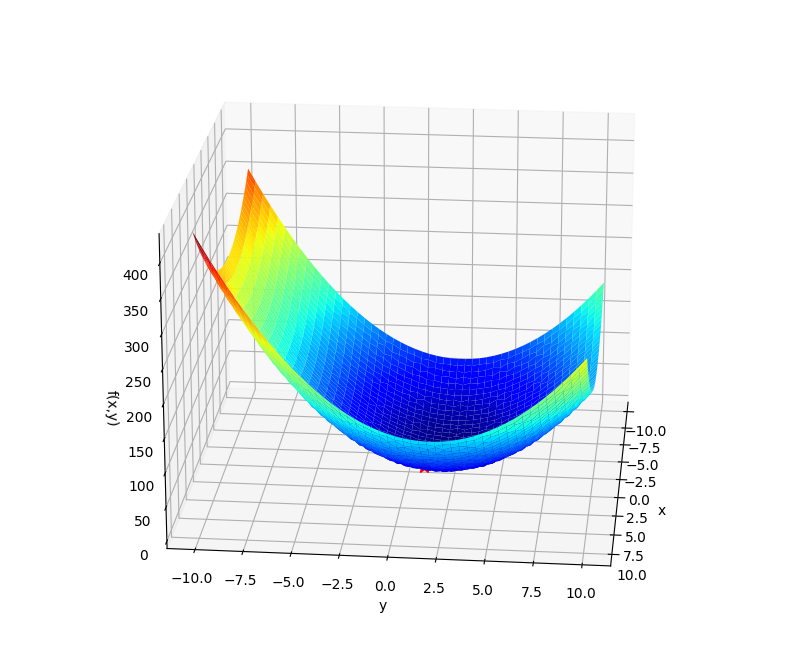
\includegraphics[width=77mm]{img/Figure_1_21.png}}
	\subfigure[Vista ampliada en una región]{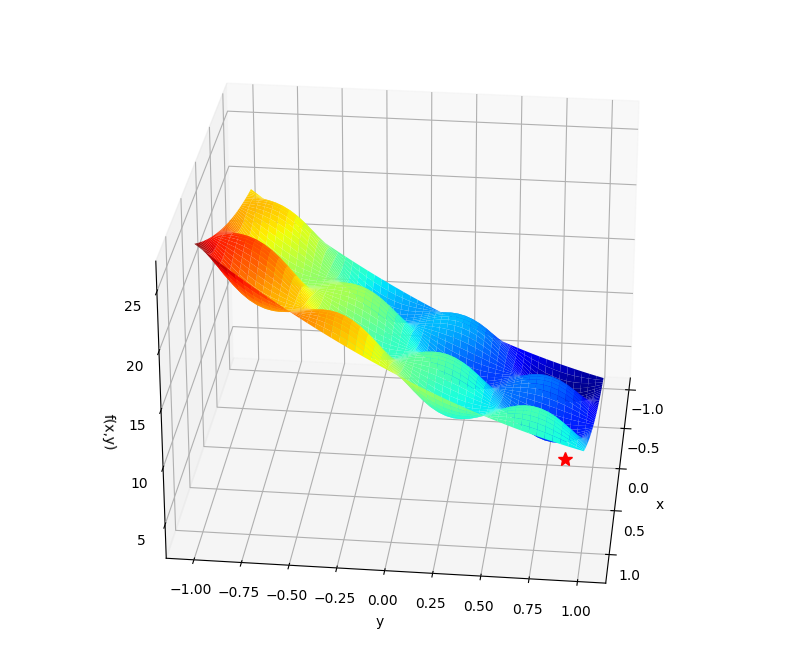
\includegraphics[width=77mm]{img/Figure_1_2.png}}
	\caption{}
	\label{fig:f(x,y)}
\end{figure}

Podemos ver que la función presenta una gran cantidad de mínimos locales, por lo que el algoritmo de gradiente descendente puede quedar atrapado en cualquiera de ellos.

Tenemos que el gradiente de $f(x,y)$ es:

\begin{align*}
\nabla f(x,y) & = (\frac{\partial f}{\partial x}(x,y),\frac{\partial f}{\partial y}(x,y))=\\
& = (2(x+2)+4\pi\cos(2\pi x)\sin(2\pi y),4(y-2)+4\pi\sin(2\pi x)\cos(2\pi y))
\end{align*}

definido en el código por la función \lstinline|gradf|.

Usamos la función \lstinline| plot_gd(init,f,grad,maxIter,lr)|, que implementa el algoritmo del gradiente descendente y además genera una gráfica con la evolución de los valores de la función a la que se aplica el algoritmo. La ejecutamos para la función $f(x,y)$ dada en el ejercicio y su gradiente \lstinline|gradf|, con los parámetros especificados en el enunciado. Las gráficas obtenidas para los dos valores del learning rate pedidos han sido las siguientes:

\begin{figure}[H]
    \centering    
    \subfigure[$\eta=0.01$]{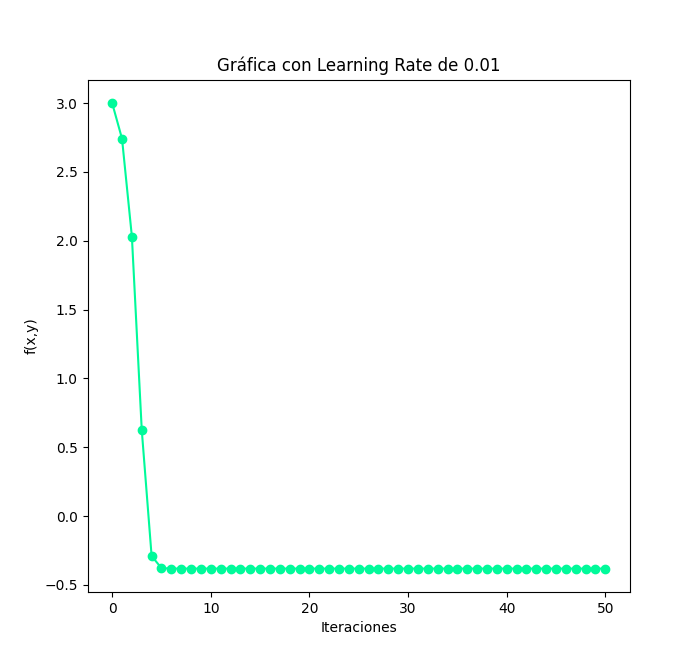
\includegraphics[width=77mm]{img/Figure_2.png}}
    \subfigure[$\eta=0.1$]{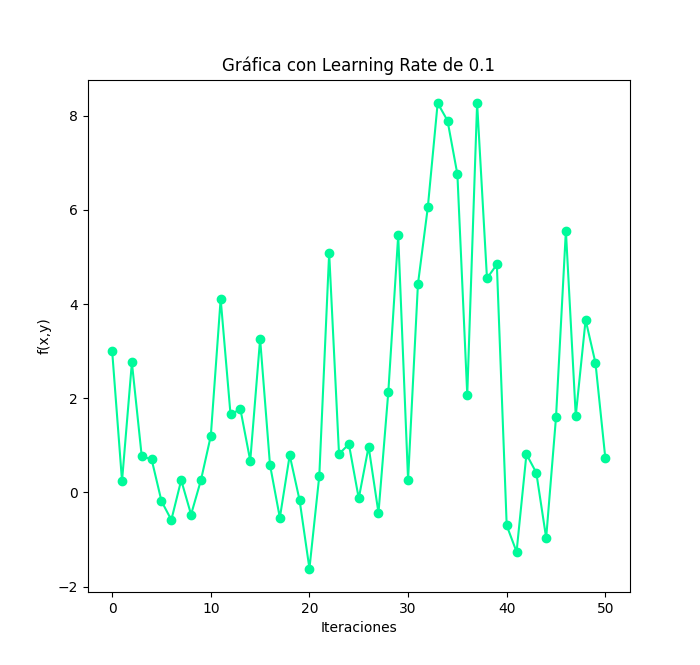
\includegraphics[width=77mm]{img/Figure_3.png}}
    \caption{}
    \label{fig:comp-eta}
\end{figure}

Observamos que para una tasa de aprendizaje relativamente pequeña, $\eta=0.01$, los valores de la función van disminuyendo progresivamente en cada iteración y el algoritmo converge bastante rápido a un mínimo de la función, que no es el mínimo global, pues vemos en la seguna gráfica que la función puede tomar valores menores que $-0.5$. Es decir, el algoritmo queda atrapado en un mínimo local y no es capaz de encontrar el mínimo absoluto. Sin embargo, para $\eta=0.1$, el algoritmo no converge a ningún mínimo, sino que los valores de la función van oscilando. Esto ocurre porque esta tasa de aprendizaje es demasiado grande y el algoritmo se salta los puntos donde se alcanzan los mínimos, de manera que los valores de la función pueden volver a crecer.

En general, se tiene que para una tasa de aprendizaje pequeña el algoritmo converge casi seguramente a un mínimo, que no tiene por qué ser el mínimo global de la función, esto es, se puede quedar atascado en un mínimo local no muy bueno. Además, cuanto más pequeña sea la tasa de aprendizaje, más lenta es la convergencia. En cambio, si esta es grande, la convergencia es más rápida, pero puede ocurrir que el algoritmo no encuentre un mínimo, sino que se lo salte cuando esté cerca de él y llegue a un punto donde la función toma valores mayores. 

Por lo tanto, es importante elegir bien este parámetro para que se encuentre un mínimo suficientemente bueno y en un número razonable de iteraciones. 
\subsubsection{Apartado b)}

\textbf{Obtener el valor mínimo y los valores de las variables $(x, y)$ en donde se alcanzan
cuando el punto de inicio se fija en: $(-0.5, -0.5),(1, 1), (2.1, -2.1),(-3, 3),-2, 2)$.
Generar una tabla con los valores obtenidos. Comentar la depenpendecia del punto
inicial.}

Para este caso consideramos la función \lstinline|gd(init,f,grad,maxIter,lr)|, que simplemente implementa el algoritmo de gradiente descendente y realiza tantas iteraciones como indique el parámetro \lstinline|maxIter|. Es decir, para cuando se alcanza el máximo número de iteraciones y no cuando la función tome un determinado valor, como ocurría en la función  \lstinline|gradient_descent)| usada para el ejercicio 2, ya que no sabemos en este caso cuál es el mínimo absoluto. Esto también lo hace la función \lstinline|plot_gd|, pero ahora no se representa nada gráficamente.

Así pues, llamamos a esta función con \lstinline|maxIter=50| y \lstinline|lr=0.01| (pues ya hemos visto que con esta tasa de aprendizaje y número de iteraciones se encuentra un mínimo, aunque no sea el global), partiendo de los distintos puntos que se indican en el enunciado y obtenemos los siguientes resultados:

\begin{table}[H]
	\centering
	\caption{}
	\begin{tabular}{|c|c|c|}
		\hline
		\textbf{Punto inicial } & \textbf{(x,y) donde se alcanza el mínimo} & \textbf{f(x,y)} \\ \hline
		(-0.5,-0.5) &  ( -0.7934994705090673 , -0.12596575869895063 ) & 9.12514666290186 \\ \hline
		(1,1) &  ( 0.6774387808772109 , 1.290469126542778 ) & 6.43756959886592 \\ \hline
		(2.1,-2.1) &  ( 0.14880582855887767 , -0.09606770499224294 ) & 12.490971442685 \\ \hline
		(-3,3) &  ( -2.7309356482481055 , 2.7132791261667037 ) & -0.3812494974381 \\ \hline
		(-2,2) &  ( -2.0 , 2.0 ) & -4.7992313045179e-31 \\ \hline
	\end{tabular}
	\label{}
\end{table}

\vspace{-5mm}
Nos damos cuenta de que  distintos puntos de partida nos llevan a diferentes mínimos locales de la función, que pueden ser mejores o peores. 
El punto inicial $(-3,3)$ es el que nos conduce al mejor de los mínimos locales, pues el valor de la función en el punto encontrado es el más bajo de todos. Para los puntos $(-0.5,-0.5),(1,1),(2.1,-2.1)$, los mínimos locales encontrados son bastante malos, el algoritmo se queda atrapado en mínimos locales con valores altos. Notamos que en $(-2,2)$ la función tiene un mínimo local, pues el algoritmo de gradiente descendente no avanza y devuelve el propio punto de partida.

Podemos concluir entonces que, el encontrar un mínimo local bueno o incluso el mínimo absoluto, depende fuertemente del punto del que parte el algoritmo. 

\subsection{Ejercicio 4}
\textbf{¿Cuál sería su conclusión sobre la verdadera dificultad de encontrar el mínimo
global de una función arbitraria?}

Después de los estudios realizados en los ejercicios anteriores, queda claro que la dificultad reside en elegir correctamente la tasa de aprendizaje y el punto de partida a usar en el algoritmo del gradiente descendente. 

Si la función es convexa y presenta un único mínimo, este algoritmo encuentra fácilmente el mínimo global. Esto es lo que ocurría en el ejercicio 2, en el que la función $E(u,v)$ tenía un único mínimo y el algoritmo convergía rápidamente a éste. Sin embargo, cuando las funciones presentan muchos mínimos locales (como es el caso de la función del ejercicio 3), el algoritmo de gradiente descendente puede quedar atrapado en cualquiera de ellos, puesto que dicho algoritmo sólo tiene en cuenta información local de la función, o incluso puede no converger a ningún mínimo si la tasa de aprendizaje es muy alta. Es necesario entonces seleccionar la tasa de aprendizaje y punto inicial que nos lleven al mínimo global, lo cual no es tarea sencilla, pues dependen de la forma de la función.

En la práctica no podemos visualizar siempre las funciones para ver qué forma tienen, como hemos hecho en los ejercicios anteriores, (por ejemplo si dependen de más de dos parámetros), por lo que es difícil determinar qué tasa de aprendizaje y punto de partida son los adecuados. Habría que probar sistemáticamente con distintos valores hasta encontrar algunos que nos lleven a un mínimo suficientemente bueno para la aplicación considerada. 
\newpage
\section{Ejercicio sobre regresión lineal}
\textbf{Este ejercicio ajusta modelos de regresión a vectores de características extraidos de imágenes
de digitos manuscritos. En particular se extraen dos características concretas que miden: el valor
medio del nivel de gris y la simetría del número respecto de su eje vertical. Solo se seleccionarán
para este ejercicio las imágenes de los números 1 y 5.
}
\subsection{Ejercicio 1}
\textbf{Estimar un modelo de regresión lineal a partir de los datos proporcionados por
los vectores de características (intensidad promedio y simetría) usando tanto el algoritmo
de la pseudo-inversa como el Gradiente descendente estocástico (SGD). Las etiquetas serán
$\{-1, 1\}$, una por cada vector de cada uno de los números. Pintar las soluciones obtenidas
junto con los datos usados en el ajuste. Valorar la bondad del resultado usando $E_{in}$ y
$E_{out}$ (para $E_{out}$ calcular las predicciones usando los datos del fichero de test).
}

Empezamos viendo el \textbf{algoritmo de Gradiente Descendente Estocástico (SGD)}. 
Este algoritmo divide el conjunto de datos original en subconjuntos aleatorios (batches o mini-batches) de un determinado tamaño indicado por el programador (tamaño de mini-batch) sobre los que se aplica el algoritmo de gradiente descendente. En cada iteración se considera un subconjunto diferente hasta que se cubre todo el conjunto de datos (el último subconjunto puede tener un tamaño menor al del resto de batches, dependiendo de si el tamaño del dataset completo es un múltiplo o no del tamaño de batch). En ese caso, se vuelven a dividir los datos en nuevos subconjuntos donde volver a aplicar el algoritmo. Este proceso se repite hasta alcanzar un determinado número de iteraciones, parámetro también establecido por el programador. 

En un modelo de regresión lineal, la función que se busca minimizar es el error cuadrático medio, que viene dado por la expresión:

$$ E_{in}(w)=\frac{1}{N}\|Xw-Y\|^2$$

donde $N$ es el número de datos de entrenamiento, X es el conjunto de características de los datos de entrenamiento, Y son sus correspondientes etiquetas y w es el vector de pesos que caracterizan a una función lineal, la cual buscamos determinar. En nuestro caso, X es una matriz donde cada fila contiene un 1 junto con las características de intensidad promedio y simetría de un dígito, e Y es un vector con la etiqueta 1 (para el dígito 5) o -1 (para el dígito 1) asociada a un dato en cada posición. Esta función está definida en el código en \lstinline|Err(w)|.

El gradiente de la función de error, que usaremos en el algoritmo de gradiente descendente, es:
$$\nabla E_{in}(w)=\frac{2}{N} X^T(Xw-Y)$$

En esta práctica he implementado este algoritmo como sigue:
\begin{lstlisting}[language=Python]
SGD:
	w = 0
	indices = shuffle indices de X
	indice batch = 0
	for i in range(max_iteraciones):
		final batch= indice batch + tam_batch
		x = X[indices[indice batch : final batch]]
		y = Y[indices[indice batch : final batch]]
		gradiente_error = 2*x.T*(x*w-y)/N #Los productos son matriciales
		w = w - learning_rate*gradiente_error
		indice batch = final batch
		
		if indice batch >= longitud de indices:
			indices = shuffle indices de X
			indice batch = 0

	return w
 	
\end{lstlisting}
 cuyo código se puede encontrar en la función \lstinline|sgd(x,y,lr,maxIter,minibatch_size)|.
% Se parte del vector de pesos inicializados a 0 y de un vector con los índices del conjunto de datos X permutados aleatoriamente. En cada % iteración, se queda con los datos de X e Y que se encuentran en las posiciones indicadas por los elementos del vector de índices que 
 
Llamamos a esta función con un una tasa de aprendizaje de 0.01 (\lstinline|lr|), pues ya vimos en los ejercicios anteriores que daba resultados aceptables, y con un total de 1000000 iteraciones (\lstinline|maxIter|). Además, vamos a analizar los resultados que se obtienen para distintos tamaños de batch. Tamaños de batch típicos son las potencias de 2 (16,32,64,128,256,...), por lo que probaremos con ellos, además de para tamaño 1 (que nos da el algoritmo de gradiente descendente estocástico puro) y tamaño igual al de todo el conjunto de datos, es decir, en cada iteración del algoritmo de gradiente descendente se usa el dataset completo y no un subconjunto del mismo (lo que se conoce como Batch Gradient Descent). Los valores del error en la muestra y el error en el conjunto de test, así como el vector de pesos solución, obtenidos se pueden ver en la siguiente tabla:

\begin{table}[htbp]
	\centering
	\caption{Comparación de SGD para distintos tamaños de batch}
	\begin{tabular}{|c|c|c|c|}
		\hline
		\textbf{Tamaño de batch} & \textbf{Ein} & \textbf{Eout} & \textbf{Vector de pesos} \\ \hline
		1 (SGD) & 0.142656698795787 & 0.222391391591675 & (-1.09287681, -1.24694876, -0.57672583) \\ \hline
		16 & 0.079236345263511 & 0.130404673862512 & (-1.11595326, -1.24904664, -0.49519536) \\ \hline
		32 & 0.079256587243787 & 0.131760833340641 & (-1.11651933, -1.24866565, -0.50051806) \\ \hline
		64 & 0.079314425142637 & 0.130144482707188 & (-1.11701312, -1.24820566, -0.49397247) \\ \hline
		128 & 0.079349296405783 & 0.130060148854707 & (-1.1168939,  -1.25092165, -0.49363416) \\ \hline
		256 & 0.079339630509784 & 0.132181988587119 & (-1.11537984, -1.25372038, -0.50192582) \\ \hline
		Tamaño de X (BGD) & 0.079186586289004 & 0.130953837200529 & (-1.11588016, -1.24859546, -0.49753165) \\ \hline
	\end{tabular}
	\label{}
\end{table}

\vspace{-2mm}

Podemos observar que los resultados varían ligeramente según el tamaño de batch. El algoritmo de Batch Gradient Descent obtiene los mejores resultados en el conjunto de entrenamiento. En el caso en que se usa un único dato en cada iteración del algoritmo, los resultados son peores. Esto es debido a que los resultados van oscilando mucho en cada iteración y puede no llegar a converger a un buen mínimo, pues quizás necesitaría más iteraciones y un learning rate menor. Para un tamaño de Batch=128 se tiene el valor más bajo del error en el conjunto de test.

 Estos resultados dependen de los subconjuntos aleatorios seleccionados en el algoritmo y en este caso se obtienen para una semilla de 1, por lo que pueden cambiar si se fija otra semilla. Es decir, puede ser que al tomarse otros subconjuntos aleatorios, se obtengan mejores resultados para un tamaño de 32, por ejemplo, que para un tamaño de 128. Es muy probable que en nuestro caso estas diferencias mínimas en los resultados se deban a la aleatoriedad de los subconjuntos seleccionados más que al propio tamaño del batch, y para todos los casos los resultados son bastante buenos, por lo que podríamos decir que este parámetro no es muy imporante en nuestro problema concreto. Lo que sí se puede asegurar, puesto que en Batch Gradient Descent no se usan subconjuntos aleatorios de los datos, es que este presenta esos valores de error en la muestra y en el conjunto de test independientemente de la semilla fijada. 

En general, se tiene que para tamaños de mini-batch grandes, se necesitan menos iteraciones para converger, pero se puede caer en un mínimo local malo. Para tamaños de mini-batch más pequeños, el tiempo de convergencia es mayor y se van produciendo más oscilaciones durante el proceso, aunque, con un número suficiente de iteraciones y un learning rate adecuado, el algoritmo termina convergiendo a un óptimo local normalemtne mejor que para tamaños grandes. \\
(\underline{Referencias:} explicaciones de teoría y curso de Andrew Ng sobre redes neuronales).

Por otro lado, nos damos cuenta de que los errores en el conjunto de test son mayores que en el conjunto de entrenamiento, lo cual era esperable, pues los datos de test no han sido usados para el entrenamiento y el algoritmo no los 'ha visto' antes. Sin embargo, la diferencia no es muy grande, es de algo más de 0.05, por lo que el ajuste lineal realizado es aceptable.

%A partir de ahora vamos a tomar como tamaño de batch 128 datos, pues ha ofrecido los mejores resultados en el conjunto de test, lo que significa que la función lineal aproximada obtenida es la que actúa mejor sobre la población. El vector de pesos resultante en este caso ha sido:
%$$w=(-1.1168939,  -1.25092165, -0.49363416)$$

Para visualizar el hiperplano solución obtenido con este algoritmo junto con los datos de entrenamiento, he usado la función \lstinline|plot_plano3d(w,x,y,title,axis_labels,legend_labels)|, cuyo código está escrito siguiendo el tutorial de \href{https://likegeeks.com/3d-plotting-in-python/ }{https://likegeeks.com/3d-plotting-in-python/ }, la documentación oficial de las funciones empleadas, así como algunos detalles que aparecen en \\
\href{https://stackoverflow.com/questions/20505105/add-a-legend-in-a-3d-scatterplot-with-scatter-in-matplotlib}{https://stackoverflow.com/questions/20505105/add-a-legend-in-a-3d-scatterplot-with-scatter-in-matplotlib} y\\
 \href{https://stackoverflow.com/questions/12904912/how-to-set-camera-position-for-3d-plots-using-python-matplotlib}{https://stackoverflow.com/questions/12904912/how-to-set-camera-position-for-3d-plots-using-python-matplotlib}.
 
 Las solución obtenida para tamaño de batch de 128, por ejemplo (para los otros tamaños la solución varía tan poco que no se aprecia en la representación gráfica) ha sido la siguiente:
 
 \begin{figure}[H]
 	\centering
 	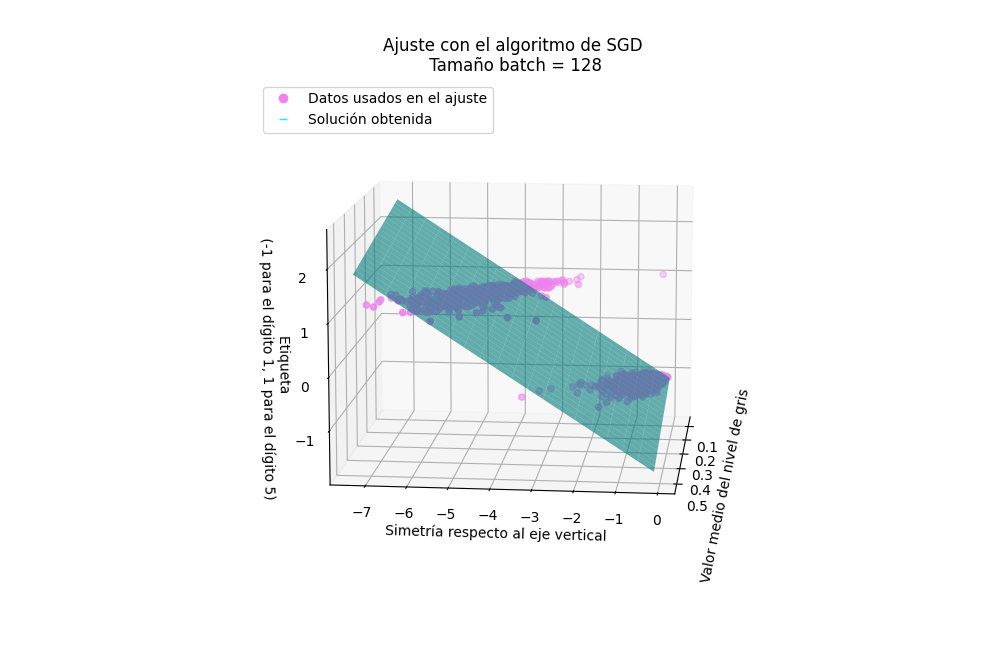
\includegraphics[width=1.1\linewidth]{img/tam128}
 	\caption{}
 	\label{fig:tam16}
 \end{figure}
 \vspace{-2mm}
  Pasamos ahora a estudiar el \textbf{algoritmo de la Pseudo-inversa}. Este algoritmo nos da siempre los valores óptimos de los pesos, es decir, determina la función lineal que mejor se ajusta a los datos de entrenamiento. Consiste en igualar el gradiente del error cuadrático (ya visto antes) a 0 y despejar de la fórmula obtenida el vector de pesos w:
  $$\nabla E_{in}(w)=\frac{2}{N} X^T(Xw-Y)=0 \rightarrow X^TXw=X^TY \\ \rightarrow w=((X^TX)^{-1})X^TY$$
  donde $((X^TX)^{-1})X^T$ es la matriz pseudo-inversa de X. 
 
 Así pues, nuestro algorimto consiste simplemente en calcular la matriz pseudo-inversa de X y multiplicarla por el vector de etiquetas Y, que es exactamente lo que se hace en la función \lstinline|pseudoinverse(x,y)|.
 
La solución obtenida por este algoritmo se visualiza a continuación:
 
   \begin{figure}[H]
  	\centering
  	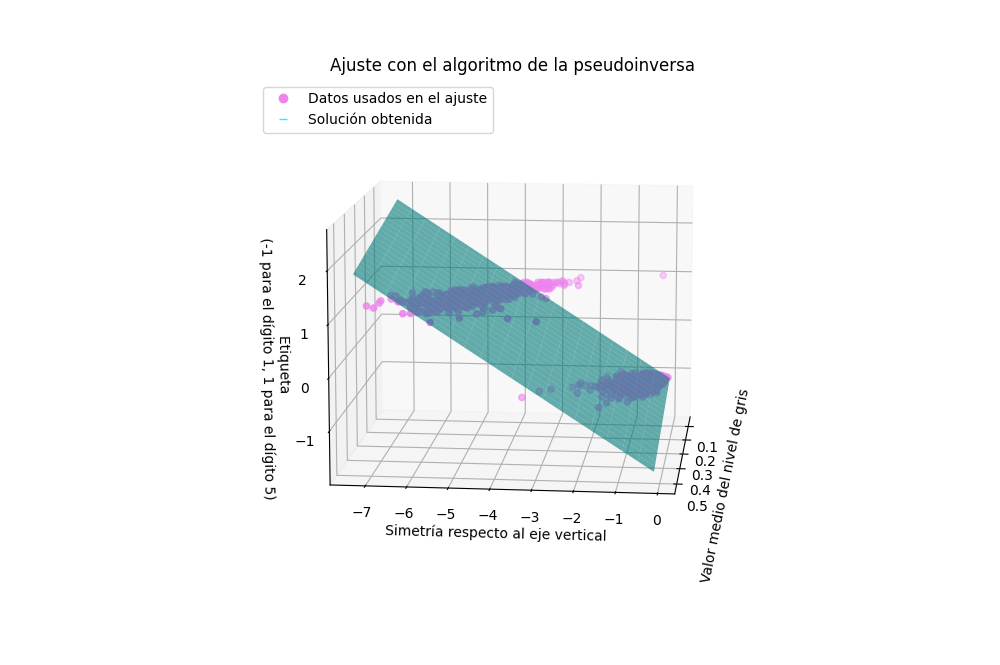
\includegraphics[width=1.1\linewidth]{img/pseudoinversa}
  	\caption{}
  	\label{fig:pseudo-inversa}
  \end{figure}
\vspace{-2mm}

que se corresponde con los siguientes pesos: $w=(-1.11588016, -1.24859546, -0.49753165)$

Comparamos ahora los errores obtenidos con este algoritmo y los obtenidos con el algorimto de SGD: 

\begin{table}[htbp]
	\centering
	\caption{Comparación de la bondad de los algoritmos}
	\begin{tabular}{|c|c|c|}
		\hline
		& \textbf{Ein} & \textbf{Eout} \\ \hline
		\textbf{Pseudo-Inversa} & 0.079186586289004 & 0.130953837200526 \\ \hline
		\textbf{BGD} & 0.079186586289004 & 0.130953837200529 \\ \hline
		\textbf{SGD tam=16} & 0.079236345263511 & 0.130404673862512 \\ \hline
		\textbf{SGD tam=32} & 0.079256587243787 & 0.131760833340641 \\ \hline
		\textbf{SGD tam=64} & 0.079314425142637 & 0.130144482707188 \\ \hline
		\textbf{SGD tam=128} & 0.079349296405783 & 0.130060148854707 \\ \hline
		\textbf{SGD tam=256} & 0.079339630509784 & 0.132181988587119 \\ \hline
		\textbf{SGD tam=1} & 0.142656698795787 & 0.222391391591675 \\ \hline
	\end{tabular}
	\label{}
\end{table}

\vspace{-2mm}

Como era de esperar, en la muestra el algoritmo de la pseudo-inversa ofrece los mejores resultados, ya que siempre encuentra la solución óptima, lo cual no está asegurado con el SGD. Sin embargo, en este caso vemos que el algoritmo de Batch Gradient Descent alcanza el óptimo, pues sus errores coinciden con los del algorimto de la pseudo-inversa. Con los otros tamaños de batch (a excepción de 1), el algoritmo se queda bastante cerca del óptimo, converge en una buena dirección. Con un número más elevado de iteraciones es posible que también hubiera encontrado el valor mínimo. Así, para este problema, no es necesario usar tamaños de batch más pequeños, pues con todo el conjunto de datos se encuenta el valor óptimo y en menos iteraciones.

Si nos fijamos en el error en el conjunto de test, este es algo inferior para algunos tamaños de batch con el algoritmo de SGD (como 128) que con la pseudo-inversa. Esto es debido a que el algoritmo de la pseudoinversa nos da una solución que se adapta perfectamente a los datos de entrenamiento, pero esta solución no tiene por qué ser la mejor para el resto de la población y, en particular, para el conjunto de test. 
%La solución que ofrece el SGD es un poco peor para los datos de la muestra porque no se ajusta tanto a ellos, pero generaliza mejor para otros datos desconocidos de la población. 

Mostramos finalmente una representación en 2D con los datos de entrenamiento y las soluciones obtenidas por cada algoritmo, para lo cual hemos hecho uso de la función \\ \lstinline|plot_plano2d(x,y,title,lim,axis_labels,legend_labels,*w)| (su implementación y demás detalles pueden verse en el código):

\begin{figure}[H]
	\centering
	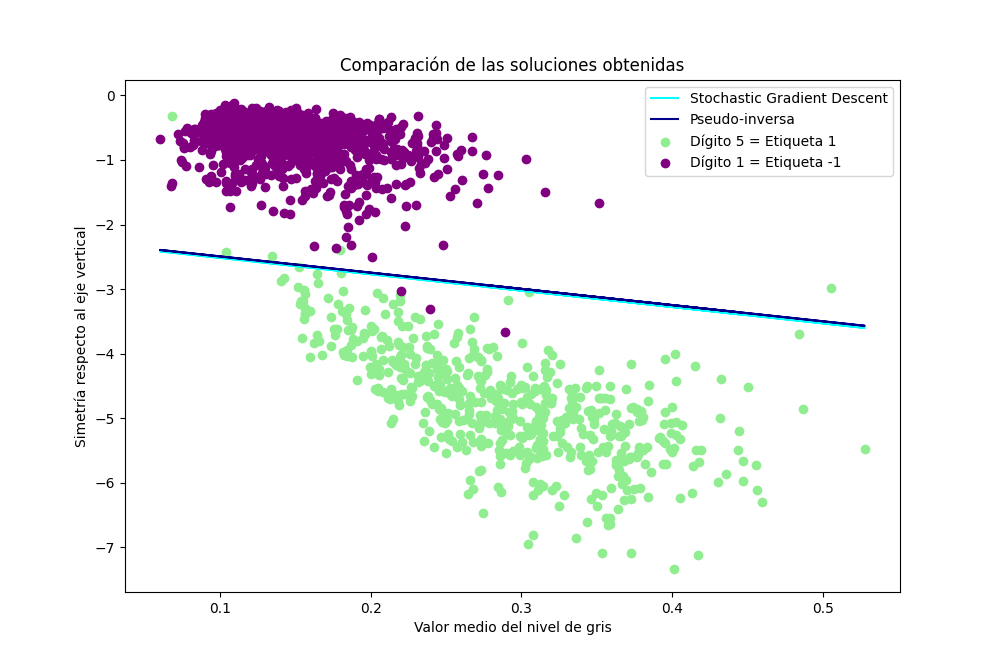
\includegraphics[width=1\linewidth]{img/comparacion}
	\caption{}
	\label{fig:comparacion}
\end{figure}
\vspace{-2mm}

Se puede apreciar que ambos algoritmos separan bastante bien los datos de las dos clases de que disponemos
%, y la solución que nos da SGD coincide casi totalmente con la que nos da la pseudo-inversa.


\subsection{Ejercicio 2}

\textbf{En este apartado exploramos como se transforman los errores $E_{in}$ y $E_{out}$ cuando
aumentamos la complejidad del modelo lineal usado. Ahora hacemos uso de la función
$simula unif (N, 2, size)$ que nos devuelve N coordenadas 2D de puntos uniformemente
muestreados dentro del cuadrado definido por $[-size, size] \times [-size, size]$.}

\subsubsection{Apartado a)}

\textbf{Generar una muestra de entrenamiento de $ N = 1000 $ puntos en el cuadrado\\
$ X = [-1, 1] \times [-1, 1] $. Pintar el mapa de puntos 2D.}

Usamos la función \lstinline|simula_unif| con N=1000 puntos, d=2 dimensiones y size=1, para simular 1000 puntos uniformemente muestreados en el cuadrado $[-1, 1] \times [-1, 1] $. Representamos gráficamente los puntos obtenidos y el resultado es:

\begin{figure}[H]
	\centering
	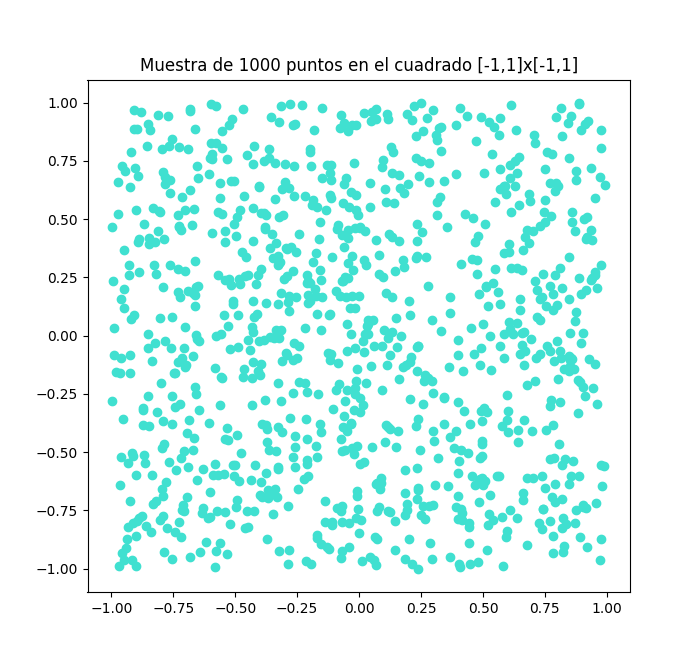
\includegraphics[width=0.8\linewidth]{img/Figure_7}
	\caption{}
	\label{fig:figure7}
\end{figure}

\subsubsection{Apartado b)}
\textbf{Consideremos la función $f (x_1 , x_2 ) = sign((x_1 - 0,2)^2 + x_2^2 - 0.6)$ que usaremos
para asignar una etiqueta a cada punto de la muestra anterior. Introducimos
ruido sobre las etiquetas cambiando aleatoriamente el signo de un 10 \% de las
mismas. Pintar el mapa de etiquetas obtenido.}

En el código, definimos la función dada en \lstinline|f(x1, x2)|, que usamos para asignar etiquetas a los puntos de la muestra antes creada (se le asigna un 1 o -1 a cada elemento de la muestra) y nos creamos un vector con estas etiquetas. Para introducir el ruido, lo que hacemos es crear un vector con algunos de los índices del vector de etiquetas seleccionados aleatoriamente y con un tamaño igual al 10\% de la longitud del vector de etiquetas. Después simplemente cambiamos el signo de las etiquetas que ocupen las posiciones indicadas por los elementos del vector de índices aleatorios. 

Visualizamos los datos de la muestra asignando un color diferente a los que pertenecen a distintas clases (tienen distintas etiquetas) y obtenemos la siguiente figura:

\begin{figure}[H]
	\centering
	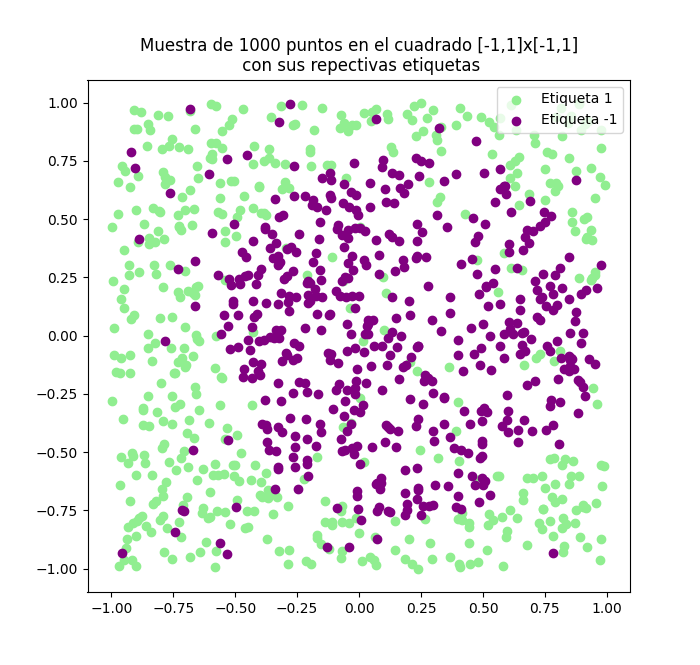
\includegraphics[width=0.8\linewidth]{img/Figure_8}
	\caption{}
	\label{fig:figure8}
\end{figure}

\subsubsection{Apartado c)}
\textbf{Usando como vector de características $(1, x_1 , x_2 )$ ajustar un modelo de regresion
lineal al conjunto de datos generado y estimar los pesos $ w $. Estimar el error de
ajuste $ E_{in} $ usando Gradiente Descendente Estocástico (SGD).}

En primer lugar, para obtener el conjunto de vectores de características, añadimos un 1 a cada par de coordenadas $(x_1,x_2)$ de la muestra generada. Una vez hecho esto, podemos aplicar el algoritmo de gradiente descendente estocástico (ya explicado en el ejercicio anterior e implementado en la función \lstinline|sgd|) a este conjunto de vectores de características y a sus correspondientes etiquetas (obtenidas en el apartado anterior). Lo ejecutamos para una tasa de aprendizaje de 0.01 como venimos haciendo hasta ahora, 10000 iteraciones y un tamaño de mini-batch de 32 por ejemplo (pues ya hemos visto que para nuestros datasets sencillos este parámetro no influye demasiado).  El vector de pesos obtenido ha sido: $w=( 0.0952433,  -0.55563738, -0.02589885) $ \\
que presenta un error en la muestra de $Ein:  0.8827608910998747$

Si visualizamos en 3D los datos de la muestra junto con la solución obtenida, como hicimos en el ejercicio anterior usando la función \lstinline|plot_plano3d|, obtenemos:

\begin{figure}[H]
	\centering
	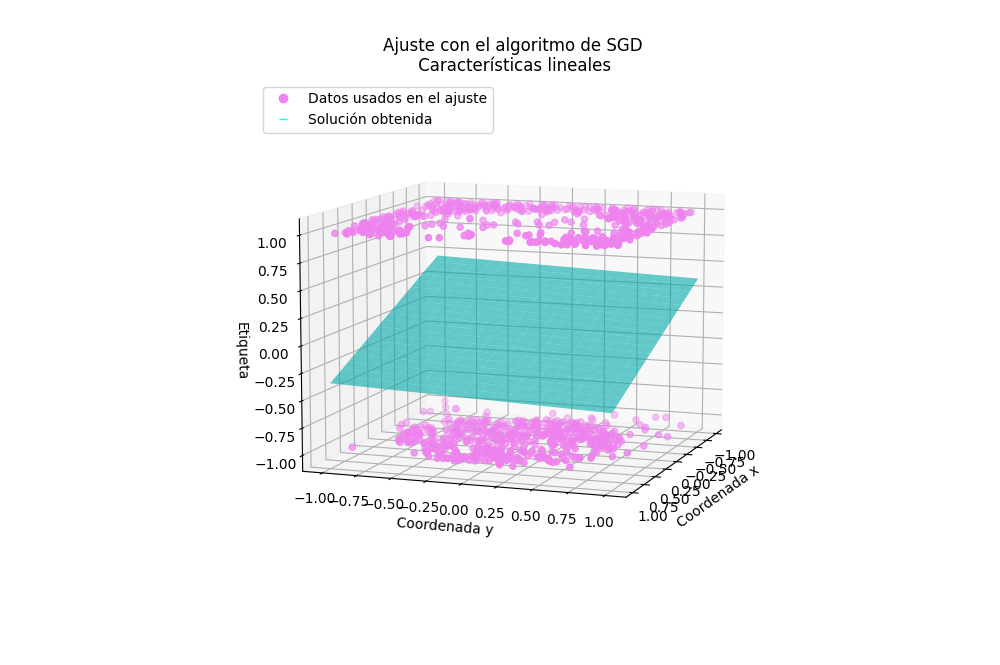
\includegraphics[width=1.1\linewidth]{img/Figure_9_lin}
	\caption{}
	\label{fig:figure9lin}
\end{figure}

y si proyectamos en el plano $Z=0$ esta solución (función \lstinline|plot_plano2d|) observamos lo siguiente:

\begin{figure}[H]
	\centering
	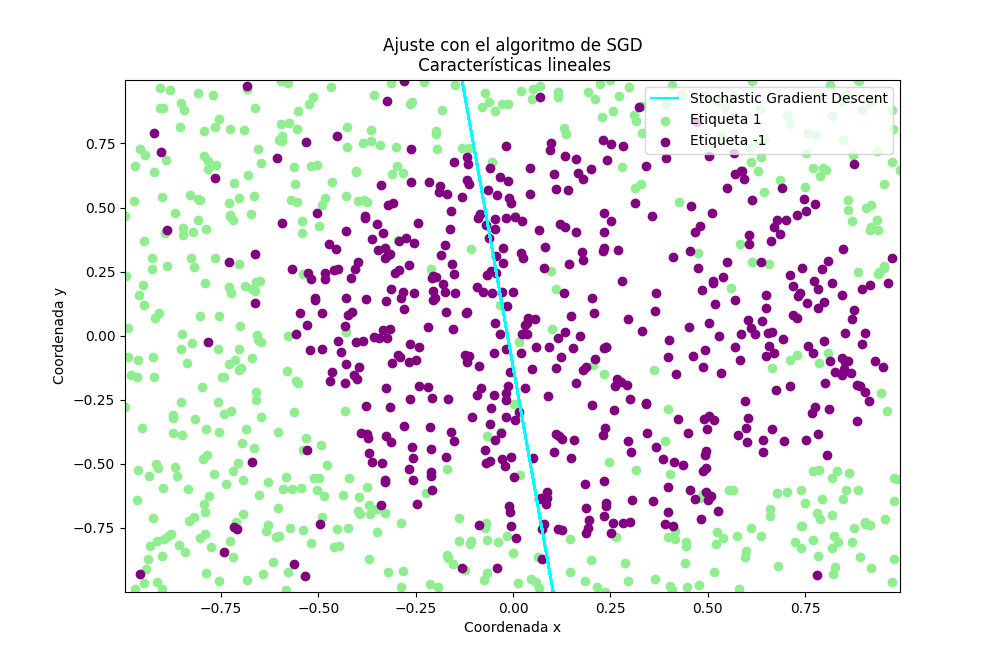
\includegraphics[width=0.9\linewidth]{img/Figure_10}
	\caption{}
	\label{fig:figure10}
\end{figure}


\subsubsection{Apartado d)}
\textbf{Ejecutar todo el experimento definido por (a)-(c) 1000 veces (generamos 1000
muestras diferentes) y
\begin{itemize}
	\item Calcular el valor medio de los errores $ E_{in} $ de las 1000 muestras.
	\item Generar 1000 puntos nuevos por cada iteración y calcular con ellos el valor
	de $ E_{out} $ en dicha iteración. Calcular el valor medio de $ E_{out} $ en todas las
	iteraciones.
\end{itemize}}

Para este apartado consideramos la función \lstinline|datos()| que lleva a cabo los pasos seguidos en los apartados anteriores: generación de la muestra, asignación de etiquetas a los datos de la misma, introducción de ruido en las etiquetas y creación de los vectores de características. 	

Lo que hacemos es generar 1000 muestras de entrenamiento y otras 1000 muestras de test llamando a esta función. Aplicamos el algorimto de gradiente descendente estocástico (con los parámetros especificados en el apartado anterior) a cada muestra de entrenamiento, sumamos los errores asociados a los pesos obtenidos por el algoritmo para cada muestra (sumamos por separado tanto $E_{in}$ como $E_{out}$, calculando este último sobre la muestra de test) y los dividimos entre 1000 (es decir, hacemos la media de $E_{in}$ y $E_{out}$ de todas las muestras generadas). Los resultados obtenidos tras llevar esto a cabo han sido los siguientes:
\begin{center}
$E_{in}$ medio: 0.9225920957871286 \\
$E_{out}$ medio: 0.9291867775786113
\end{center}

\subsubsection{Apartado e)}
\textbf{Valore que tan bueno considera que es el ajuste con este modelo lineal a la vista
de los valores medios obtenidos de $E_{in}$ y $E_{out}$}

Podemos ver que los errores medios son bastante altos, están muy cercanos a 1, tanto en la muestra como en los conjuntos de test generados, lo cual es un indicador de que un ajuste con un modelo lineal no es lo más apropiado para este problema. Este hecho se aprecia en la Figura 10, donde podemos observar que no hay ninguna recta que permita separar adecuadamente las dos clases. Así pues, el ajuste con este modelo lineal es muy malo. 

Esto era esperable, pues la función $(x_1 - 0,2)^2 + x_2^2 - 0.6$ que permite asignar las etiquetas a los datos no es lineal, sino cuadrática, por lo que ninguna función lineal podría aproximarla de manera adecuada. En la figura 8 vemos que los datos podrían separarase con alguna elipse o circunferencia.  

\subsubsection{Ajuste con características no lineales}

\textbf{Repetir el mismo experimento anterior pero usando características no lineales. Ahora
usaremos el siguiente vector de características: $\Phi_2(x)=(1,x_1,x_2,x_1x_2,x_1^2,x_2^2)$. Ajustar el nuevo modelo de regresión lineal y calcular el nuevo vector de pesos $\hat{w}$. Calcular
los errores promedio de $E_{in}$ y $E_{out}$.
}

Empezamos generando los datos haciendo uso de la función \lstinline|datos()|, que nos devuelve un conjunto de vectores con características lineales y sus correspondientes etiquetas. Como queremos usar características no lineales, creamos otros vectores de características, partiendo de los que nos devuelve la función \lstinline|datos()|, en la forma pedida: $x=(1,x_1,x_2,x_1x_2,x_1^2,x_2^2)$. Este nuevo conjunto de características, junto con sus etiquetas, que nos da \lstinline|datos()|, es lo que usaremos para llamar a la función \lstinline|sgd|, con los mismos valores de los parámetros usados en los apartados anteriores. La solución obtenida es entonces:\\ $$w=(-0.97760039, -0.45969182,  0.03052494, -0.09006862,  1.38092721,  1.63821293)$$ vector de mayor longitud que los obtenidos en los estudios anteriores. 
Esta solución nos da ahora un error en la muestra de $E _{in}: 0.5171784871757734$.

Podemos representar gráficamente la solución en 3D y en 2D (proyectando en el plano $Z=0$), de manera parecida a cómo lo hicimos para las soluciones lineales (ver los detalles de la implementación y procedimiento seguido en el código), para obtener las siguientes figuras:

\begin{figure}[H]
	\centering    
	\subfigure[Vista en 3D de la solución]{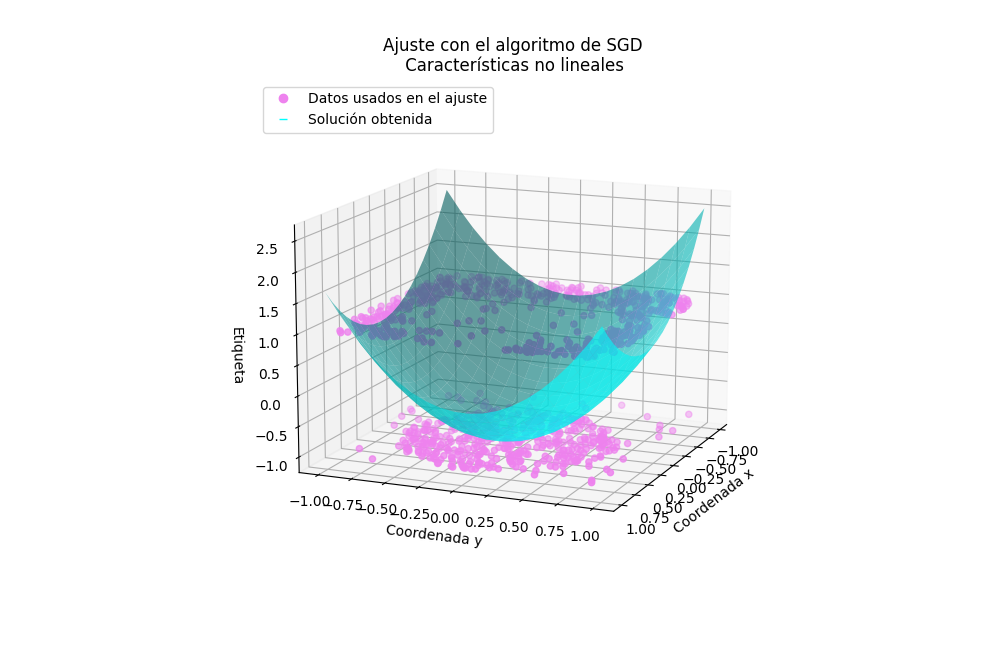
\includegraphics[width=150mm]{img/Figure_11_nolin.png}}
	\subfigure[Proyeccion de la solución en el plano $Z=0$]{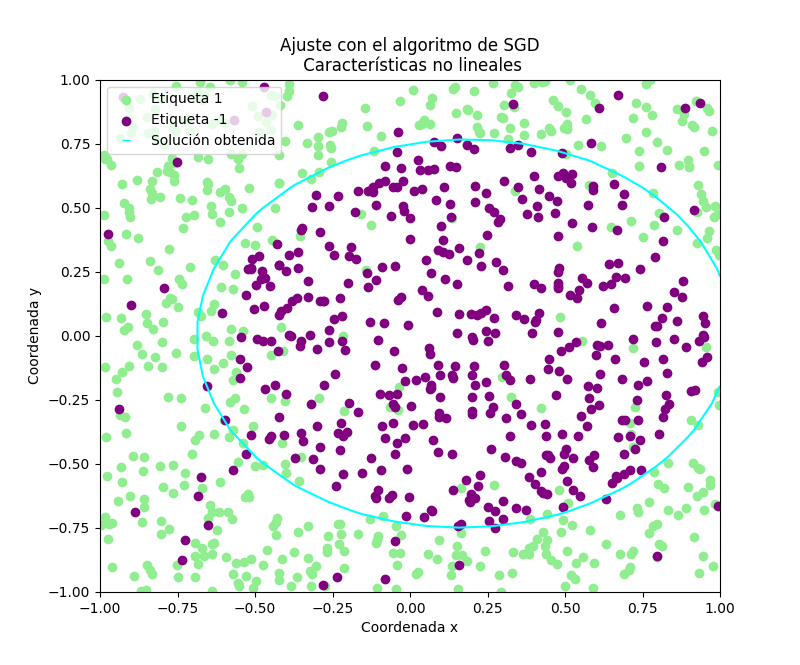
\includegraphics[width=100mm]{img/circulo.png}}
	\caption{Ajuste con características no lineales}
	\label{fig:nolin}
\end{figure}

Repetimos ahora los pasos anteriores 1000 veces (sin las representaciones gráficas), es decir, generamos 1000 muestras diferentes y le aplicamos el algoritmo de SGD para obtener distintas soluciones. Calculamos la media de los errores $E_{in}$ de las soluciones obtenidas para cada una de estas 1000 muestras y además, para cada muestra generada, creamos otra muestra de test con la que calculamos el error $E_{out}$ para la solución correspondiente a esa muestra. Hacemos también la media de todos estos errores en las 1000 repeticiones, y obtenemos lo siguiente:
\begin{center}
$ E_{in}$ medio: 0.5603409308530063 \\
$E_{out}$ medio: 0.5668512004000035 
\end{center}
\vspace{6mm}
\textbf{A la vista de los resultados de los errores promedios $ E_{in}$ y $E_{out}$ obtenidos en los dos
experimentos ¿Que modelo considera que es el más adecuado? Justifique la decisión.}

Para el caso en que consideramos características no lineales, los errores son considerablemente menores que los obtenidos cuando ajustamos un modelo con características lineales (el error se ve reducido casi un 40\%), tanto en la muestra como en el test. Así, podemos afirmar con total seguridad que el modelo que hemos ajustado usando características no lineales es el mejor para nuestro problema. En la Figura 11 apreciamos que la solución obtenida para características no lineales separa casi perfectamente los datos en sus dos clases. 

Como ya comentamos en el \textbf{apartado e)} esto es debido a que la función que asigna las etiquetas a los datos es cuadrática, por lo que es mucho más adecuado intentar aproximar esta función con características cuadráticas que con característica lineales.

\section{BONUS: Método de Newton} 

\subsection{Ejercicio 1}
\textbf{Implementar el algoritmo de minimización de Newton
y aplicarlo a la función $f (x, y)$ dada en el ejercicio 3. Desarrolle los mismos experimentos
usando los mismos puntos de inicio.
\begin{itemize}
	\item Generar un gráfico de cómo desciende el valor de la función con las iteraciones.
	\item Extraer conclusiones sobre las conductas de los algoritmos comparando la curva de
	decrecimiento de la función calculada en el apartado anterior y la correspondiente
	obtenida con gradiente descendente.
\end{itemize}}

Este algoritmo usa una regla diferente al gradiente descente para actualizar los puntos en cada iteración, basada en las segundas derivadas de la función a minimizar. En concreto hace uso de su matriz Hessiana, como sigue:
$$ w_{k+1}=w_{k}-H^{-1}\nabla f(w_k)$$ 
donde $w_{k}$ son las coordenadas obtenidas en la k-ésima iteración del algoritmo, $f$ es la función a minimizar y $H$ es la matriz Hessiana de la misma. 

El pseudo-código de este algoritmo es el siguiente:

\begin{lstlisting}[language=Python]
Metodo de Newton:
	w <-- punto inicial
	for i in range(max_iteraciones):
		w <-- (w - inv(H)*grad_f(w))
	return w
\end{lstlisting}


cuya implementanción puede encontrarse en la función \lstinline|Newton(init,f,grad,hess,maxIter)|. 

Nos piden minimizar la función $f(x,y)=(x+2)^2 +2(y-2)^2 +2\sin(2\pi x)sin(2\pi y)$ del ejercicio 3 usando este método, para lo cual debemos calcular su matriz hessiana. 

Caculamos primero las derivadas segundas de esta función, las cuales están definidas en las funciones \lstinline|fxx(w)| (= $\frac{\partial^2 f }{\partial x^2}(x,y)$), \lstinline|fyy(w)| (= $\frac{\partial^2 f }{\partial y^2}(x,y)$) y \lstinline|fxy(w)| (= $\frac{\partial^2 f }{\partial x \partial y}(x,y) = \frac{\partial^2 f }{\partial y \partial x}(x,y)$ ambas derivadas parciales coinciden por ser la función considerada de segundo orden).  Después definimos la matriz Hessiana, que para nuestra función es la siguiente:
\begin{align*}
Hess(f)= \begin{pmatrix}
\frac{\partial^2 f }{\partial x^2}(x,y) & \frac{\partial^2 f }{\partial x \partial y}(x,y) \\
\frac{\partial^2 f }{\partial x \partial y}(x,y) & \frac{\partial^2 f }{\partial y^2}(x,y)
\end{pmatrix}= 
\begin{pmatrix}
2-8\pi^2 \sin(2\pi x) \sin(2\pi y) & 8\pi^2 \cos(2\pi x) \cos(2\pi y) \\
8\pi^2 \cos(2\pi x) \cos(2\pi y) & 4-8\pi^2 \sin(2\pi x) \sin(2\pi y)
\end{pmatrix}
\end{align*}

la cual se encuentra definida en la función \lstinline|Hessf(w)|. Y ya podemos ejecutar el método llamando a \lstinline|Newton(punto,f,gradf,Hessf,maxIter)|, con nuestra función, su gradiente (ya determinado en el ejercicio 3) y su matriz hessiana. 

Para comparar los resultados con los obtenidos con el algoritmo de gradiente descendente, consideramos la función \lstinline|gd(init,f,grad,maxIter,lr)|, que básicamente implementa el algoritmo de gradiente descendente y almacena en un vector las imágenes por la función f de los puntos obtenidos en cada iteración, para poder representar luego la curva de decrecimiento de la función. 

Ejecutamos estas funciones para cada uno de los puntos iniciales dados en el apartado b) del ejercicio 3 de la primera parte de la práctica, tomando 50 iteraciones, como se indicaba en dicho ejercicio, y considerando como tasa de aprendizaje para el gradiente descentente tanto 0.1 como 0.01. A continuación, visualizamos las curvas obtenidas para cada uno de los puntos de partida y con cada uno de los algoritmo y los resultados han sido los siguientes:

\begin{figure}[H]
	\centering    
	\subfigure{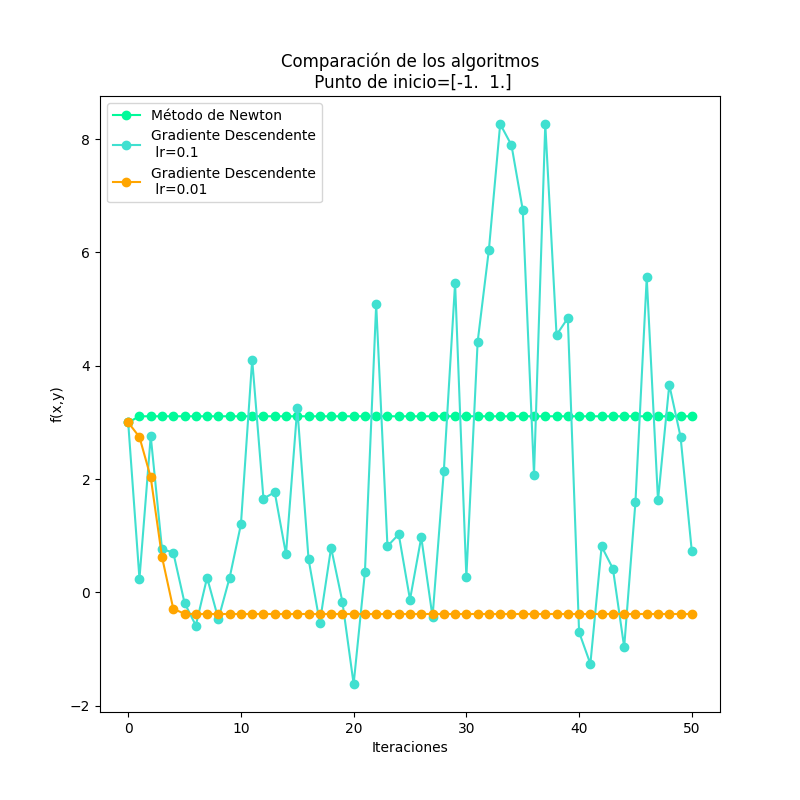
\includegraphics[width=77mm]{img/n1.png}}
	\subfigure{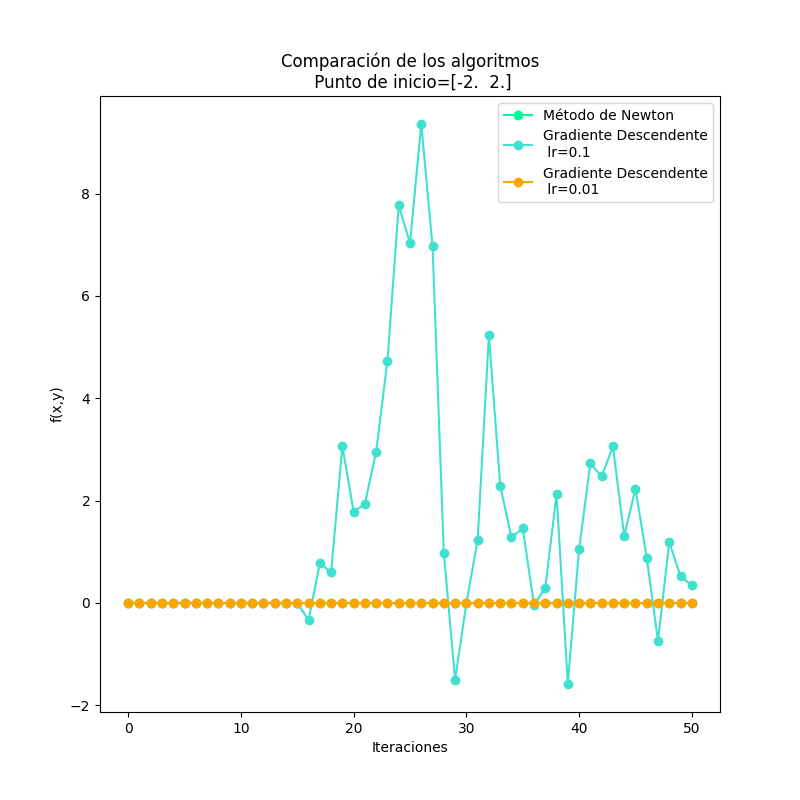
\includegraphics[width=77mm]{img/n2.png}}
	\caption{Comparación entre los algoritmos de Newton y Gradiente Descendente}
	\label{fig:new}
\end{figure}

\begin{figure}[H]
	\centering    
	\subfigure{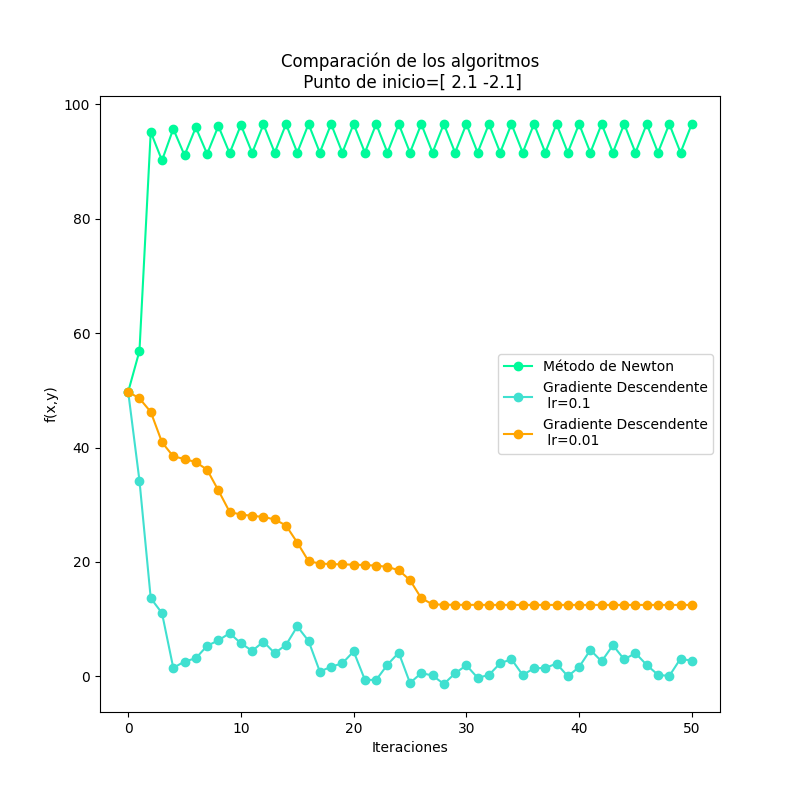
\includegraphics[width=77mm]{img/n3.png}}
	\subfigure{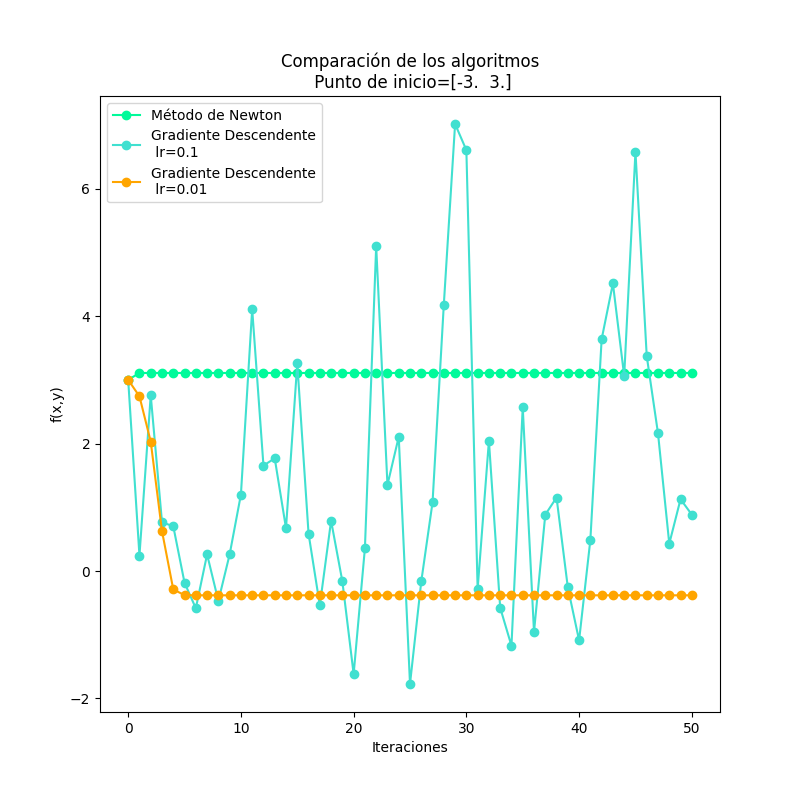
\includegraphics[width=77mm]{img/n4.png}}
	\subfigure{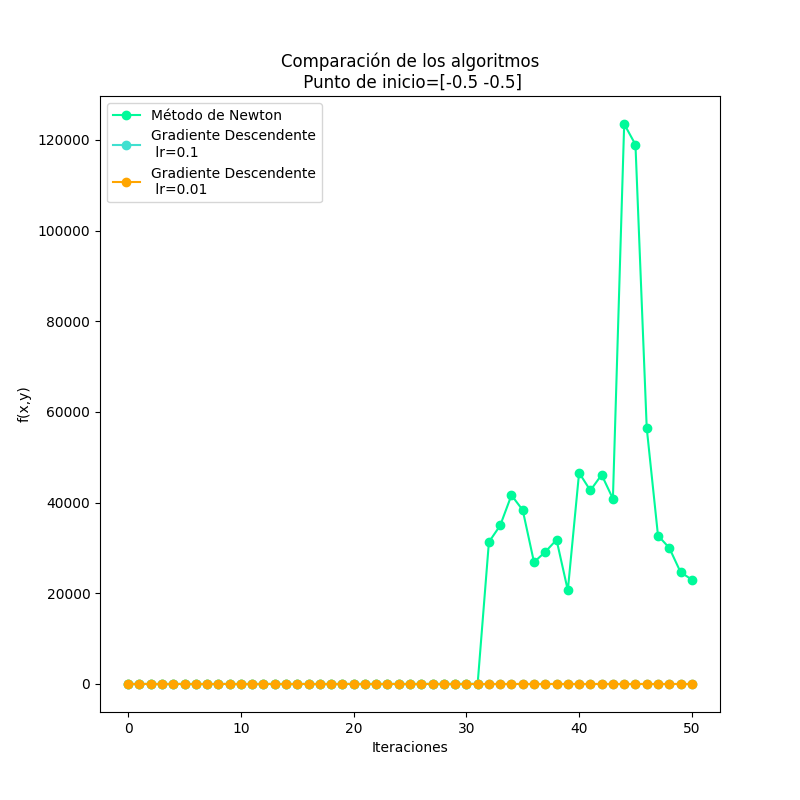
\includegraphics[width=77mm]{img/n5.png}}
	\subfigure{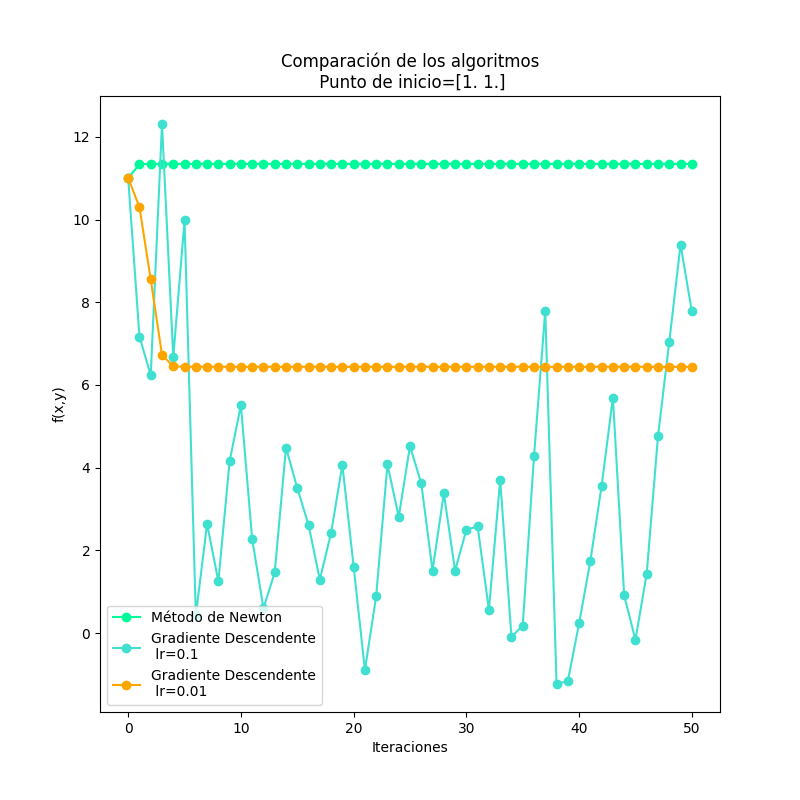
\includegraphics[width=77mm]{img/n6.png}}
	\caption{Comparación entre los algoritmos de Newton y Gradiente Descendente}
	\label{fig:new}
\end{figure}

La siguiente tabla recoje el valor de la función obtenido por el algoritmo de Newton y el punto donde se alcanza partiendo de los distintos puntos iniciales: 

\begin{table}[htbp]
	\centering
	\caption{Método de Newton con distintos puntos iniciales}
	\begin{tabular}{|c|c|c|}
		\hline
		\textbf{Punto inicial } & \textbf{(x,y) donde se alcanza el mínimo} & \textbf{f(x,y)} \\ \hline
		(-0.5,-0.5) & ( 88.41673701134395 , -84.1176167835566 ) & 23007.0011333878 \\ \hline
		(1,1) & ( 1.067372638667162 , 0.9100709200235607 ) & 11.3447557483606 \\ \hline
		(2.1,-2.1) & ( 3.8283464698659015 , -3.6596191941879828 ) & 96.5463129806446 \\ \hline
		(-3,3) & ( -3.05397555493864 , 3.028461459660191 ) & 3.1079800610352 \\ \hline
		(-2,2) &  ( -2.0 , 2.0 ) & -4.799231304517944e-31{\tiny } \\ \hline
		(-1,1) & ( -0.9460244450613605 , 0.9715385403398092 ) & 3.1079800610352 \\ \hline
	\end{tabular}
	\label{}
\end{table}



Nos damos cuenta de que el método de Newton no obtiene buenos resultados. Dependiendo del punto de partida encuentra o no un mínimo de la función. Esto es debido a que este método busca puntos críticos de la función y no sólo mínimos, que pueden ser máximos y puntos de silla. Por lo tanto, para los puntos de partida que se encuentren cerca de un máximo o punto de silla , el método tenderá a buscar esos puntos críticos en vez de un mínimo, que es lo que ocurre en los puntos de partida $(-1,1),(1,1),(-3,3)$ y $(2.1,-2.1)$ (para este punto se queda oscilando alrededor del punto crítico pero no lo alcanza). De hecho, si recordamos la forma de la función, que se puede ver en la Figura 2, notamos que tiene muchos máximos locales y puntos de silla, al igual que mínimos. Además, si durante el proceso se llega a un punto donde las derivadas segundas son muy pequeñas, la inversa de la matriz Hessiana puede llegar a dispararse y terminar en un punto totalmente alejado del mínimo. Es probable que esto es lo que ocurra  en el punto de partida $(-0.5,0.5)$. 

%Así, tenemos que si en el punto de partida la función es cóncava, este método tenderá a buscar un máximo, mientras que si es convexa sí buscará el mínimo local más cercano (que puede ser bueno o malo).
Así pues, podemos concluir que para aplicar este método es necesario partir de un punto que se encuentre bastante cerca de un mínimo, y que sepamos que es suficientemente bueno, lo cual no siempre podemos saber. En la práctica, como ya comentamos, no se conoce en la mayoría de los casos la forma de la función. 

Este método es más eficiente que el método del gradiente descendente si se aplica en el punto adecuado y necesita menos iteraciones para converger, pues usa información adicional sobre la curvatura de la función, información que no tiene en cuenta el gradiente descendente. Sin embargo, es más costoso al tener que calcular la inversa de una matriz, que puede llegar a ser muy grande si el espacio de búsqueda es de dimensión elevada. 

Este método, por lo tanto, no debe usarse como sustituto del gradiente descendente, sino sólo cuando sepamos con certeza que estamos cerca de un buen mínimo al que queremos llegar y el algoritmo de gradiente descendente no es capaz de encontrarlo con precisión. 

Podríamos haber considerado una tasa de aprendizaje también para el método de Newton, pero no es necesario solo para ver cómo se comporta el método, que es lo que queremos estudiar aquí. 
\end{document}